\chapter{Characterisation techniques (red and edge TCT)}
%\chapter{Characterisation techniques (red, edge and TPA TCT)}
% Optical measurements
\label{chap:TCT}

Characterisation of detectors both before and after irradiation is of great importance to understand the effects of radiation in silicon detectors and for trying to counteract them. Typical measurements performed include I/V and C/V curves measurements as well as light illumination using Transient Current Techniques (TCT) in any of its variants. 

The I/V and C/V are purely electrical measurements in which intensity (or capacitance) is recorded at different voltages. From the corresponding curves different detector parameters such as depletion voltage, breakdown voltage\ldots can be calculated. 

The most common optical techniques are TCT in which the silicon detector is illuminated using laser. The resulting current generated due to the drift of charge carriers inside the detector is recorded over time. This \textit{transient} currents or waveforms are later analysed and can provide information about many aspects of the detector. As with the case of C/V and I/V measurements both can be done before and after irradiation in the same manner.

In this work I/V and C/V measurements will not be considered in detail and focus will be placed on TCT measurements since these are the type of measurements that TRACS simulation software is able to reproduce. In the following sections we will explain the three main TCT techniques that are currently performed as TCT silicon detector characterisation, namely red (or normal) TCT and edge-TCT TCT. All of them share the same basic principles of illumination and signal recording but differ in key aspects that make them more suitable for characterising one type of detector or measuring one property. 
%In this work I/V and C/V measurements will not be considered in detail and focus will be placed on TCT measurements since these are the type of measurements that TRACS simulation software is able to reproduce. In the following sections we will explain the three main TCT techniques that are currently performed as TCT silicon detector characterisation, namely red (or normal) TCT, edge-TCT and Two Photon Absorption (TPA) TCT. All of them share the same basic principles of illumination and signal recording but differ in key aspects that make them more suitable for characterising one type of detector or measuring one property. 

\section{red-TCT} % (fold)
\label{sec:redTCT}

The measuring procedure for all TCT measurements is fairly similar, the main difference being the wavelength of the laser used and how the laser is point at the detector. Since silicon absorption coefficient depends on the wavelength of the light it follows that different laser frequencies will have different penetration and will yield substantially different results. All this techniques exploit the fact that photons with enough energy can create electron-hole pair that will drift inside the detector generating an electrical current. 

\begin{figure}[H]
	\centering
	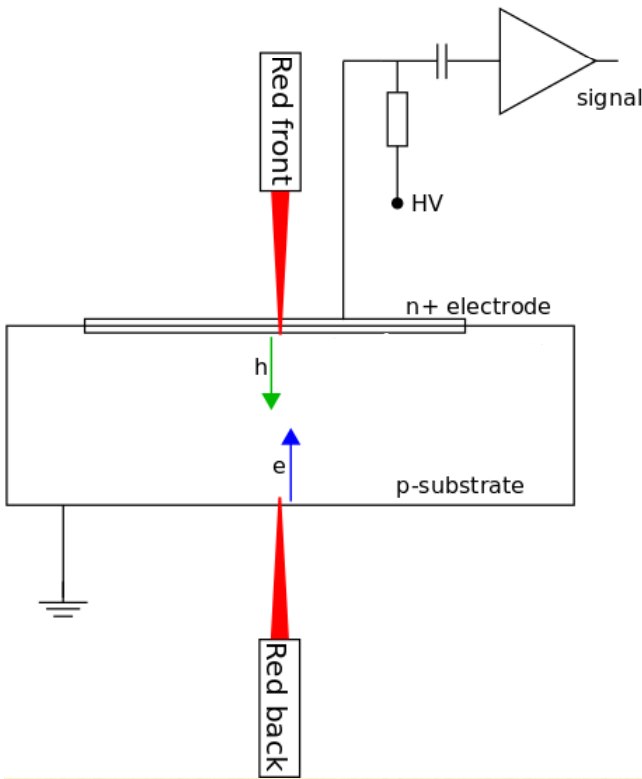
\includegraphics[width=0.6\textwidth]{chap4_redTCT.png}
	\caption{Interstitial (right) and Vacancy (left) lattice defects are illustrated here. This defects are be created inside silicon detectors after they have been irradiated.}
	\label{fig:redTCT}
\end{figure}

The most basic of TCT techniques is the so-called red-TCT. This kind of TCT measurements consist on illuminating the top or bottom part of the detector with a red laser with a typical wavelength around 660nm as shown in Figure \ref{fig:redTCT}. The absorption of these photons is a first order process since the energy of the incident photons is bigger than the minimum energy required to create an electron-hole pair. Silicon's absorption for red light is high and hence, all the photons are absorbed within a few $\mu m$ from the edge. 

All the electron-hole pairs are created in a small region very close to one of the collection electrodes. Taking top-TCT of a n-on-p diode as example, the laser is shot over the implant and barely reaches the bulk. After the charge carriers are created, the electrons are collected in less than a nanosecond contributing to signal with just a very high and narrow spike in current, usually masked off by the electronics(Bandwidth ~2.6GHz). The holes, on the other hand, drift throughout the whole bulk of the detector leaving a much longer signal. When the laser is shot on the bottom of the detector the process is inverted with holes being quickly collected and electrons drifting through the whole detector leaving the longer signal imprint.

This type of measurement allows to obtain information about the electric field by simply using Equation (\ref{eq:ramoMob}). Information about total charge collected can also be obtained easily. This information can be used to measure detector efficiency and also to compare silicon detectors before and after irradiation. The comparison of total charge collected can be performed using any of the TCT techniques.

%Integrating the full waveform the total amount of collected charge is obtained that can later be converted to the number of electron-hole pairs. Plotting collected charge against \vias yields a very good measurement of the $V_{dep}$ for (non)-irradiated detectors. 

%This method is the easiest TCT technique to perform and yields good results for most of the purposes. This technique is specially useful in silicon pad diodes with very simple geometry that usually have purpose-made optical holes to allow for top and bottom illumination. One of the biggest flaws of this TCT measurement is the inability to penetrate inside the detector bulk. It is also important to note that special features on the surface of the detector will heavily affect the output signal. A know example for this kind of behaviour are strip-detectors in which collection nodes are separated by less than 50$\mu m$ making top illumination more difficult to perform.

\section{e-TCT} % (fold)


To have a much better control on carrier placement inside the detector, a new way of illuminating a silicon was developed. The laser is moved to the side of the detector being shot on the edge of the detector (parallel to the implants and ohmic contacts) hence the '$edge$' naming convention. To increase the penetration depth of the light shot at the detector an infrared laser with wavelength around 1060nm is typically used. An schematic view of this configuration can be seen in Figure \ref{fig:eTCT}.

\begin{figure}[H]
	\centering
	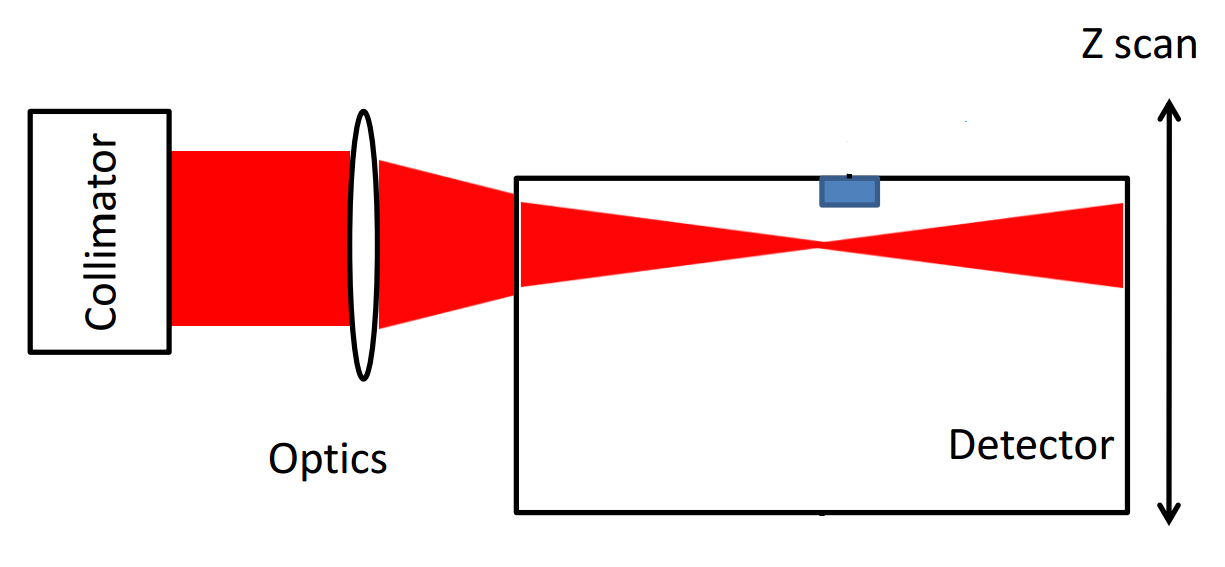
\includegraphics[width=0.8\textwidth]{chap4_eTCT.png}
	\caption{Interstitial (right) and Vacancy (left) lattice defects are illustrated here. This defects are be created inside silicon detectors after they have been irradiated.}
	\label{fig:eTCT}
\end{figure}

%In terms of the created carrier pairs, they drift in opposite directions but due to sign difference in electric charge, both current contributions add up. The final signal collected in the circuit will have too components (electrons and holes) that will give away information about the electric field in both directions. Some times it might be difficult to distinguish each component since they are both superimposed and each carrier `sees' a different field and has a different mobility. 

Typical edge-TCT scans are performed by sampling the whole detector height in steps of a couple microns and repeating this process for different \vias values.

Using this technique one can obtain the same results as using the red-TCT techniques with the additional benefit of being able to sample different parts of the detector. One can also measure the width of the depleted area for a given voltage by performing an edge-TCT scan and measuring where the total 
collected charge starts to drop. The decrease in collected charge marks the transition between the drif region and the diffusion region where the detector is not depleted. The precision of this measurement is limitted by the waist of the laser beam ($ \sigma \approx 8-10 \mu i $ m). This limitation in precision and the lack of information in the direction of the laser beam are the most notable issues with edge-TCT measuremtns.

 %\section{Two Photon Absorption - TCT} % (fold)
%
 %All the aforementioned TCT methods are first order processes in which one photon produces an electron-hole pair. The Two Photon Absorption TCT is different in this respect; TPA-TCT exploits a second order process in which two photons are responsible for a single electron-hole creation.
%
%% WIP (physical TPA process explanation)
%% Whilst typically the band gap is seen as a totally forbidden region, there's a short amount of time that electrons might be allowed to stay there, occupying a meta-stable state. The lifetime of these meta-stable states are of the order of hundreds of attoseconds and can usually be neglected. However, if one uses a fast-pulse laser, it is possible to exploit those intermediate states by sending a secondary photon before the de-excitation providing the electron with enough energy to jump to the conduction band where it reaches a stable energy level.
%
%Such a process requires the photon energy to be above half the band gap but less than the band gap energy. Fast pulse laser and high intensity of light at the region where carrier pairs should be generated are also crucial for second order processes.
%
%Since the absorption (and hence carrier generation) is proportional to the intensity of the beam squared one can play with focusing to get an abrupt transition between absorbing and non-absorbing regions. Such an abrupt transition achieved by the usage of high focusing lenses, allows for creation of really small volumes of space in which carriers will be created. 
%
 %This small volume, often called voxel, is a few microns in any direction of space allowing for 3D movement throughout the detector while maintaining good spacial resolution. Having a volume of a few cubic microns allows for very fine characterisation of the detectors and makes possible the creation of accurate 3D maps of detector properties that permit to see local imperfections or strange behaviours after irradiation.
%
 %The TPA-TCT technique is by far the most accurate one but it is still in development phase. For the moment various analysis have been performed in the laboratory using this technique with good results. Even though it is a new technique, TRACS is able to simulate such measurements provided with the correct charge carrier distribution.

 \section{Experimental setup for (red) TCT measurement} % (fold)
 \label{sec:TCTsetup}

The setup that will be described is specific for the TCT+ setup in the SSD laboratory at CERN. However, most of the TCT capable setups share most features in common so there should not be any significant difference between TCT+ setups in other laboratories. 

Only the setup for red-TCT measurements will be described for reason that will e apparent in chapter \ref{sec:TRACSvalidity}. Other TCT techniques are performed in similar manner with the main difference being the laser placement and movement.

% Equivalent circuit and SHORT expanation of material used

% Extra considerations (temperature, alignment, isolation(light and electricity)\ldots)

The whole setup is controlled via a custom LabView\cite{labview} program that also allows for remote operation and measurement. The same software takes care of saving and storing the data in the corresponding format on an ASCII file that is later analised. The data analysis procedure is performed using software specially developed in the SSD group for this purpose and that can can calculate and plot numeros physical parameters of interest such as charge collection efficiency, collection time\ldots






 
 % section Experimental setup for (red) TCT measurement (end)
